\documentclass[mathserif, 11pt, t]{beamer}
\section*{Results}

\let\Tiny=\tiny


\usepackage{graphicx}
\usepackage{float}
% \usepackage{enumitem}
\usepackage{natbib}
\usepackage{amsmath}
\usepackage{bm}
\usepackage{dsfont}
\geometry{vmargin=0.5in}


%%% Do not overwrite a defined color (#1) if already defined,
%%% otherwise set the color to rgb(#2)
\makeatletter
\newcommand{\colorprovide}[2]{%
    \@ifundefinedcolor{#1}{\definecolor{#1}{rgb}{#2}}{}}
\makeatother

%colors
\colorprovide{colorheader}{0.00, 0.40, 1.00}
\colorprovide{colortitle}{0.00, 0.24, 0.60}
\colorprovide{colorfootertext}{0.00, 0.45, 0.80}
\colorprovide{colorfooter}{0.00, 0.00, 0.00}

\setbeamercolor{local structure}{fg=colortitle}

\setbeamercolor{footlinecolor}{bg=colorfooter,fg=colorfootertext}

\beamertemplatenavigationsymbolsempty
\setbeamertemplate{footline}{%
    \hbox{%
    \vspace{0.5in}%
    \begin{beamercolorbox}[ht=2mm, rightskip=.5cm]{footlinecolor}%
    \hfill\insertframenumber/\inserttotalframenumber
    \end{beamercolorbox}}}


%\bibpunct{(}{)}{;}{a}{}{,}

%commands
\newcommand{\citei}[1]{\phantom{\cite{#1}}\vspace{-14pt}}

\newcommand{\ind}{\mathds{1}}
\newcommand{\m}[1]{\mathbf{\bm{#1}}}
\newcommand{\R}{I\hspace{-4.4pt}R}

\renewcommand{\frametitle}[1]{\vspace{0.14cm}\hspace{-0.70cm}\textcolor{colortitle}{%
    \textbf{\large{#1}}}\vspace{0.15cm}\newline}


\newcommand{\startappendix}{%
    \setbeamertemplate{footline}{%
        \hbox{%
        \vspace{0.5in}%
        \begin{beamercolorbox}[ht=2mm, rightskip=.5cm]{footlinecolor}%
        \hfill A\the\value{framenumberappendix}\phantom{/\inserttotalframenumber}
        \end{beamercolorbox}}}
    \newcounter{framenumberappendix}
    \setcounter{framenumberappendix}{0}
    }


%slide colors
\pagecolor{colorheader!60}

% title page slide
\renewcommand{\titlepage}[4]{%
    {
    \setbeamertemplate{footline}{%
        \hbox{%
        \vspace{0.5in}%
        \begin{beamercolorbox}[ht=2mm, rightskip=.5cm]{footlinecolor}%
        \phantom{/}
        \end{beamercolorbox}}}
    \begin{frame}
    %\begin{center}
    \ \\ [-0.5in]
    \vfill
    \bigskip
    \bigskip
    \bigskip
    \bigskip
    \bigskip


    %\end{center}
    \begin{Large}
    #1
    \end{Large}
    %\begin{center}
    \vfill

    #2
    \vfill

    #3
    \smallskip

    #4

    \bigskip
    \bigskip
    \vfill
    \ \\ [-0.5in]
    %\end{center}
    \end{frame}
    }
    \addtocounter{framenumber}{-1}
    }


\newcommand{\bc}[1]{\textcolor{blue}{\mathbf{#1}}}

\begin{document}


\titlepage{Comparison of extreme values of different climate model simulations and observations}{Mickey Warner}{\ }{30 Oct 2017}



\begin{frame}{Introduction}

CanCM4 simulation classes (with $R=10$ replicates each):
\begin{enumerate}
\item Decadal
\item Historical
\item Control
\end{enumerate}
\bigskip

Observations over U.S. interpolated from weather stations
\bigskip

Factors:
\begin{enumerate}
\item Variable --- Total Precipitation (\texttt{pr}) or Average Maximum Temperature (\texttt{tasmax})
\item Season --- Winter or Summer
\item Decade --- 1962--1971 or 1990--1999
\item Region --- California or USA
\end{enumerate}

\end{frame}



\begin{frame}{Locations}

\begin{figure}
\begin{center}
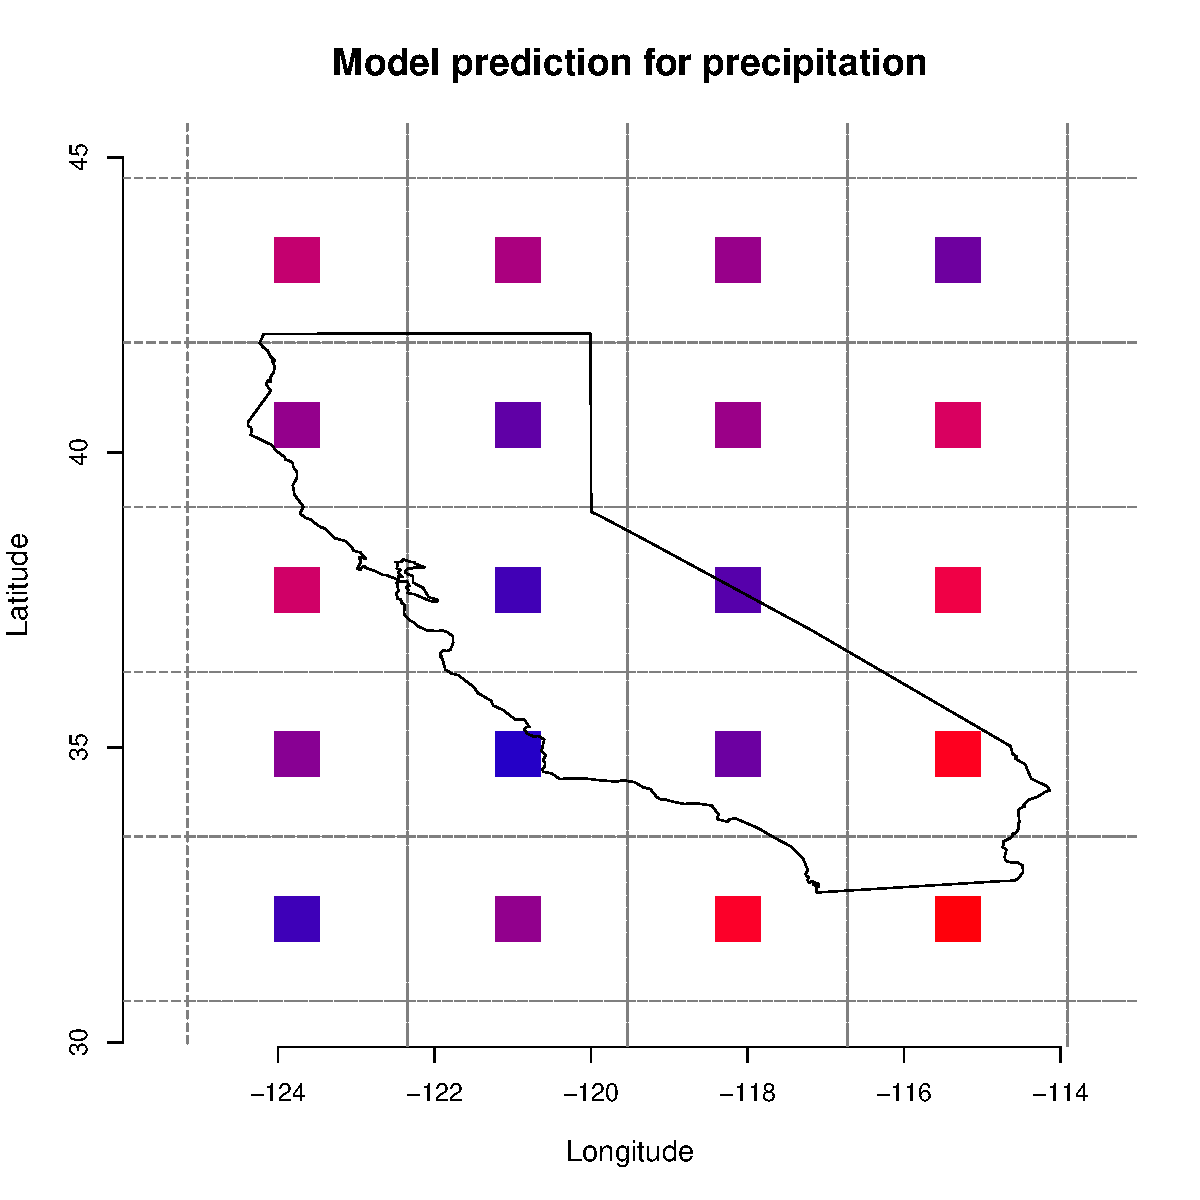
\includegraphics[scale=0.18]{figs/cal_mod_box1.pdf}
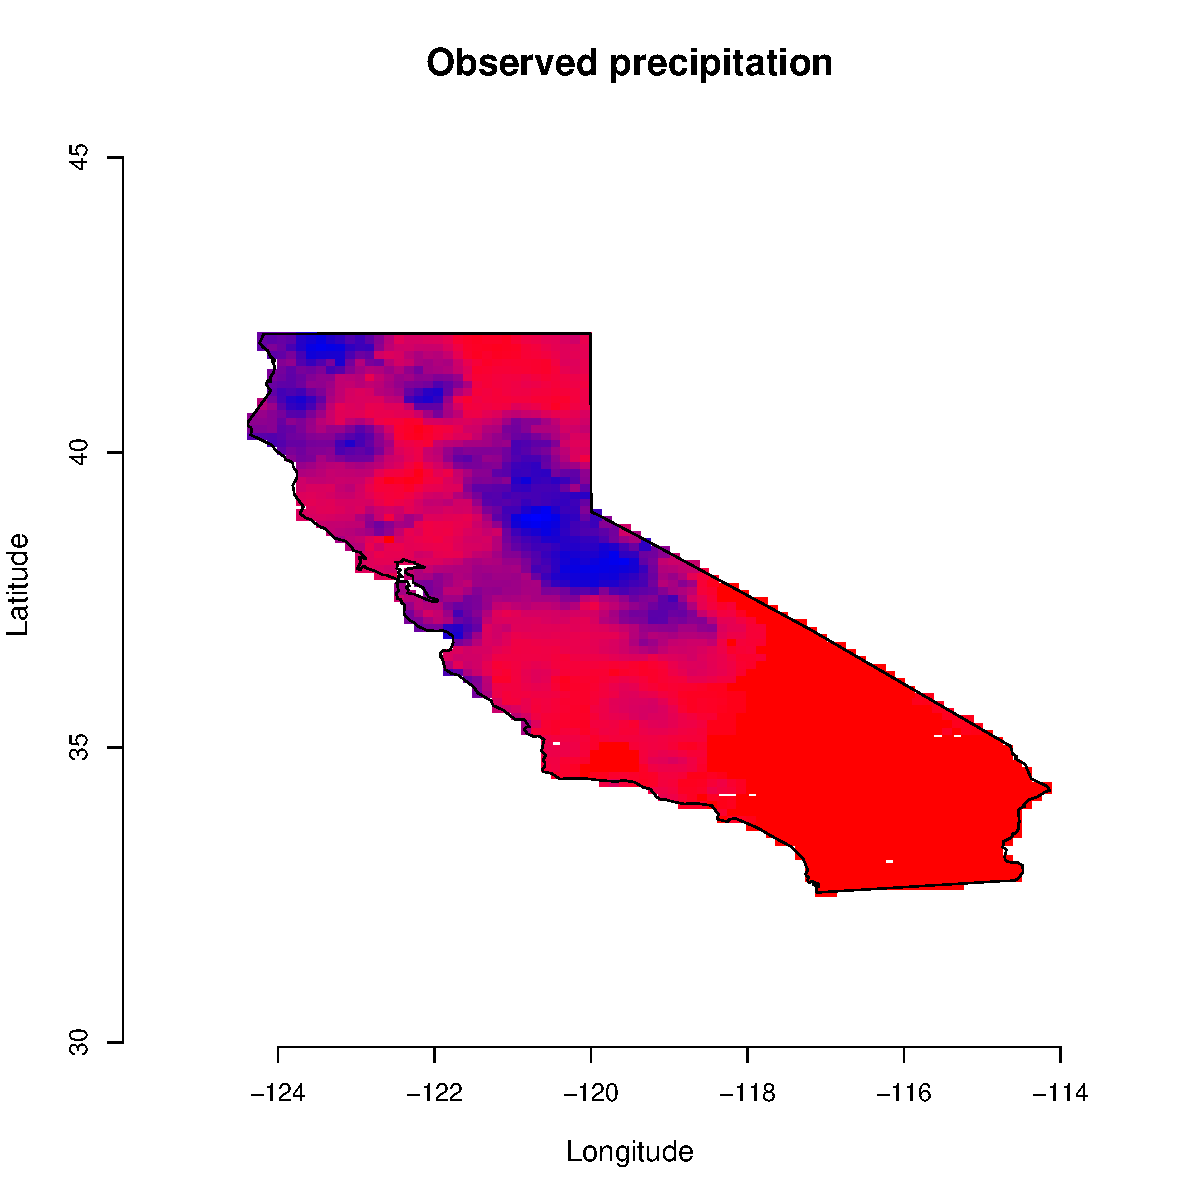
\includegraphics[scale=0.18]{figs/cal_mod_box2.pdf}
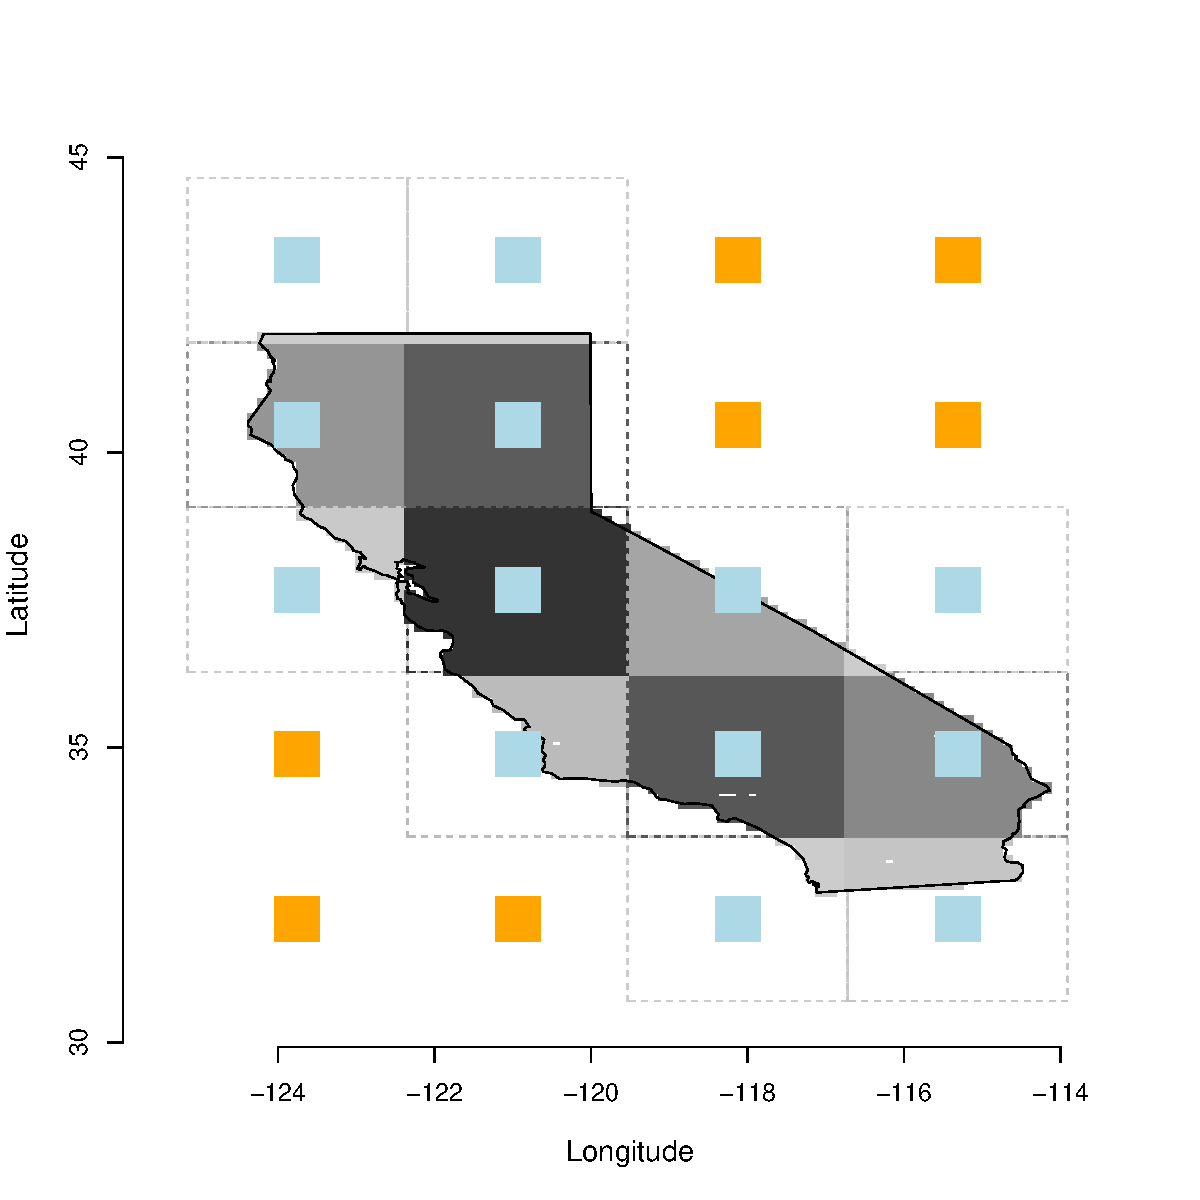
\includegraphics[scale=0.18]{figs/cal_mod_box3.pdf}
\end{center}
\caption{Left: CanCM4 simulation grid cells. Center: Observation locations. Right: method for computing weighted sum or average for CanCM4 to make values comparable with observations.}
\end{figure}

\end{frame}



\begin{frame}{Extremes}

For r.v. X and large threshold $u$, the exceedance $Y=X-u$, for $X>u$, approximately follows the generalized Pareto distribution (GPD), which has density

\[ f_Y(y) = \frac{1}{\sigma}\left(1+\xi\frac{y}{\sigma}\right)_+^{-1/\xi-1} \]

\begin{figure}
\begin{center}
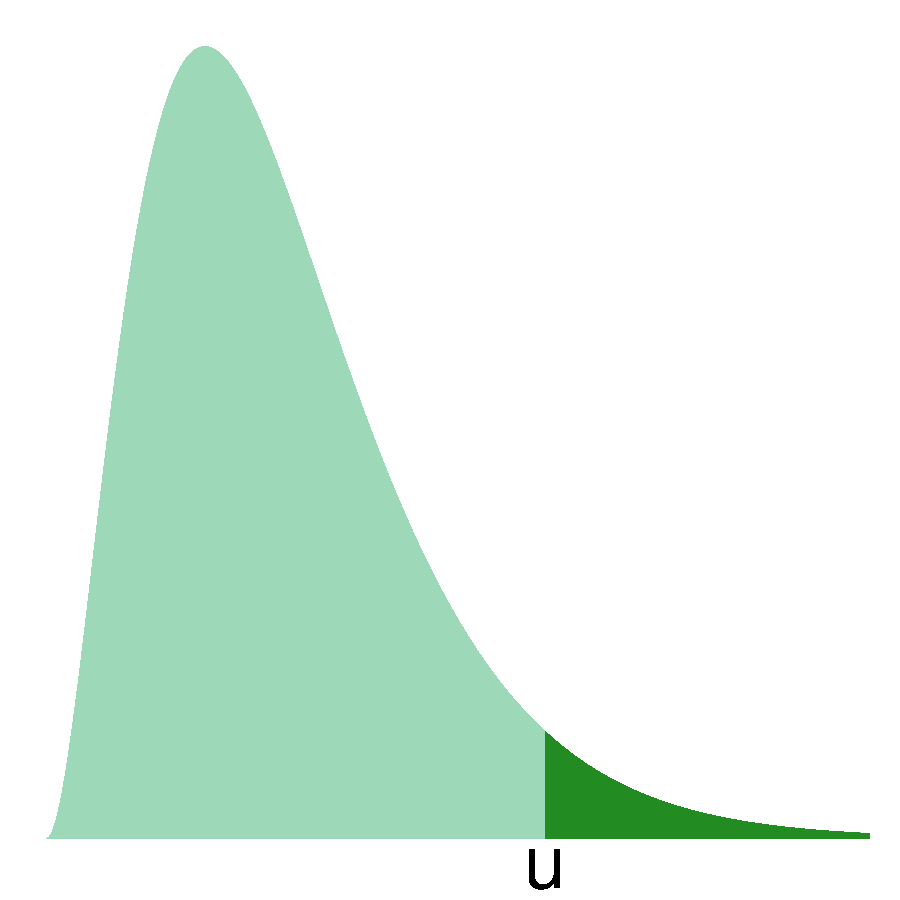
\includegraphics[scale=0.22]{figs/tail.pdf}
\end{center}
\end{figure}

\end{frame}



\begin{frame}{Data processing}

Two objectives before performing the analysis:
\begin{enumerate}
\item Make climate simulations comparable to observations
\item Get near-independent random variables for model fitting
\end{enumerate}
\bigskip

These are accomplished by
\begin{enumerate}
\item Taking weighted sums (\texttt{pr}) or weighted averages (\texttt{tasmax})
\item Computing anomalies based on DLMs, and
\item Declustering
\end{enumerate}

\end{frame}



\begin{frame}{Weighted sum or average}
\begin{figure}
\begin{center}
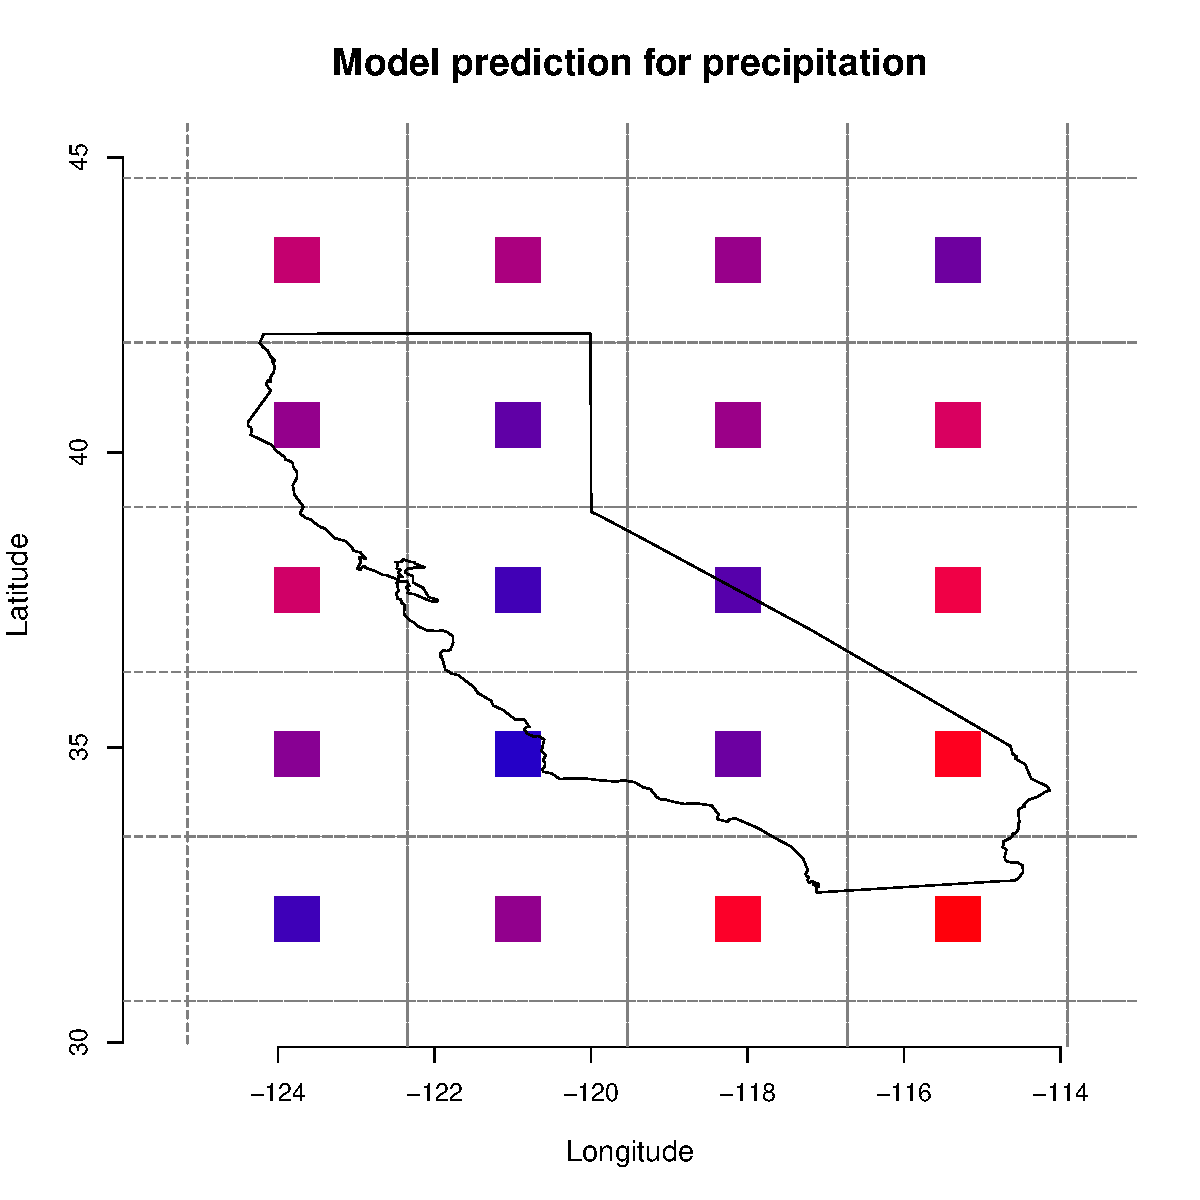
\includegraphics[scale=0.18]{figs/cal_mod_box1.pdf}
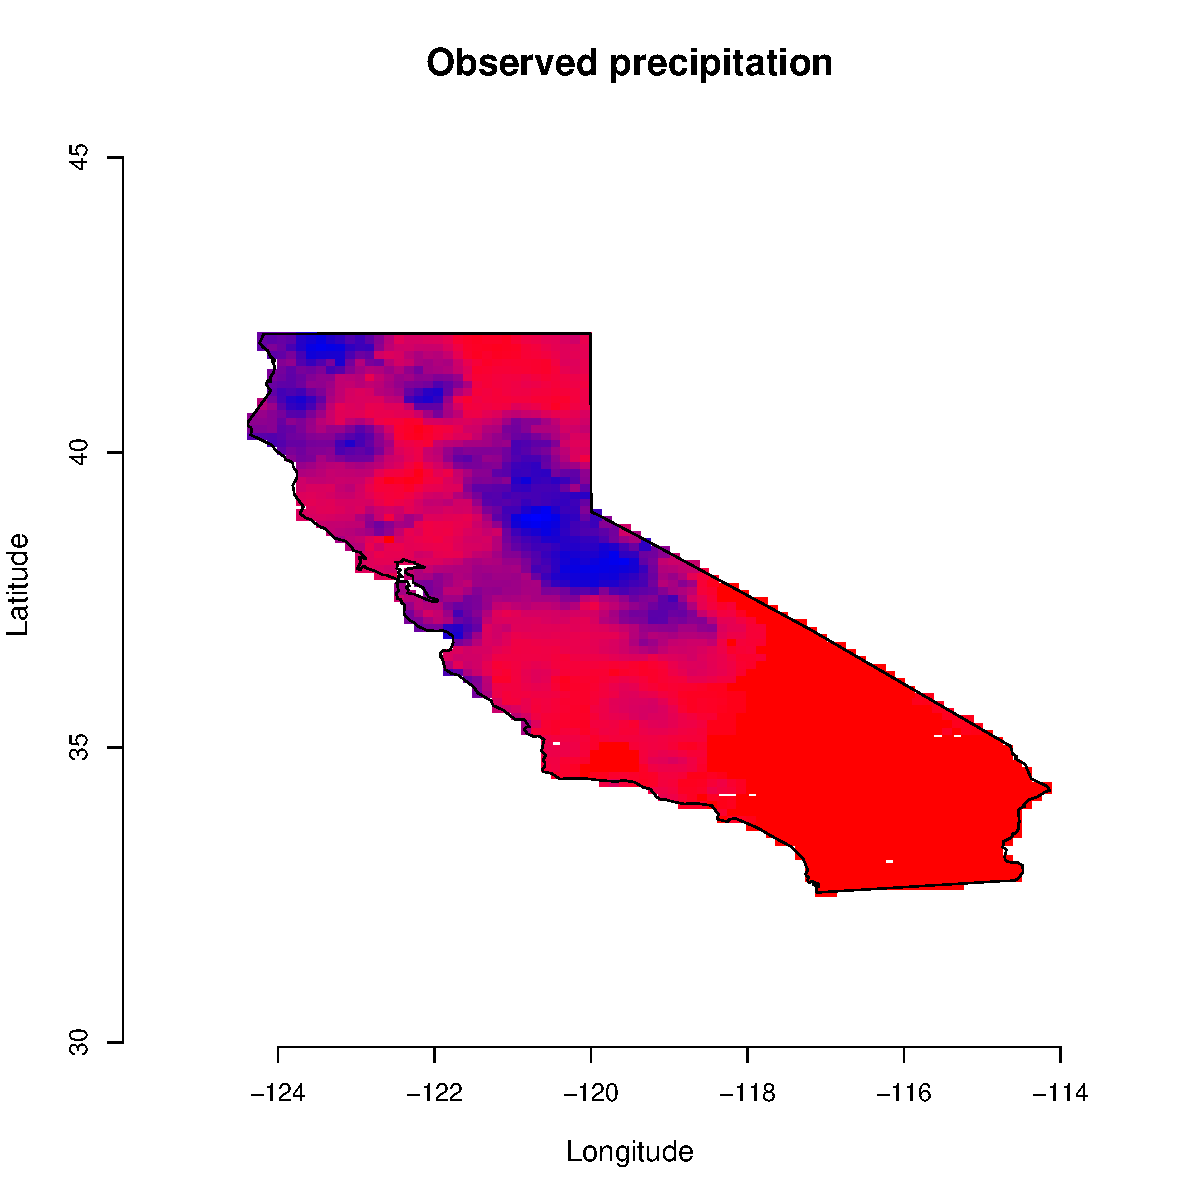
\includegraphics[scale=0.18]{figs/cal_mod_box2.pdf}
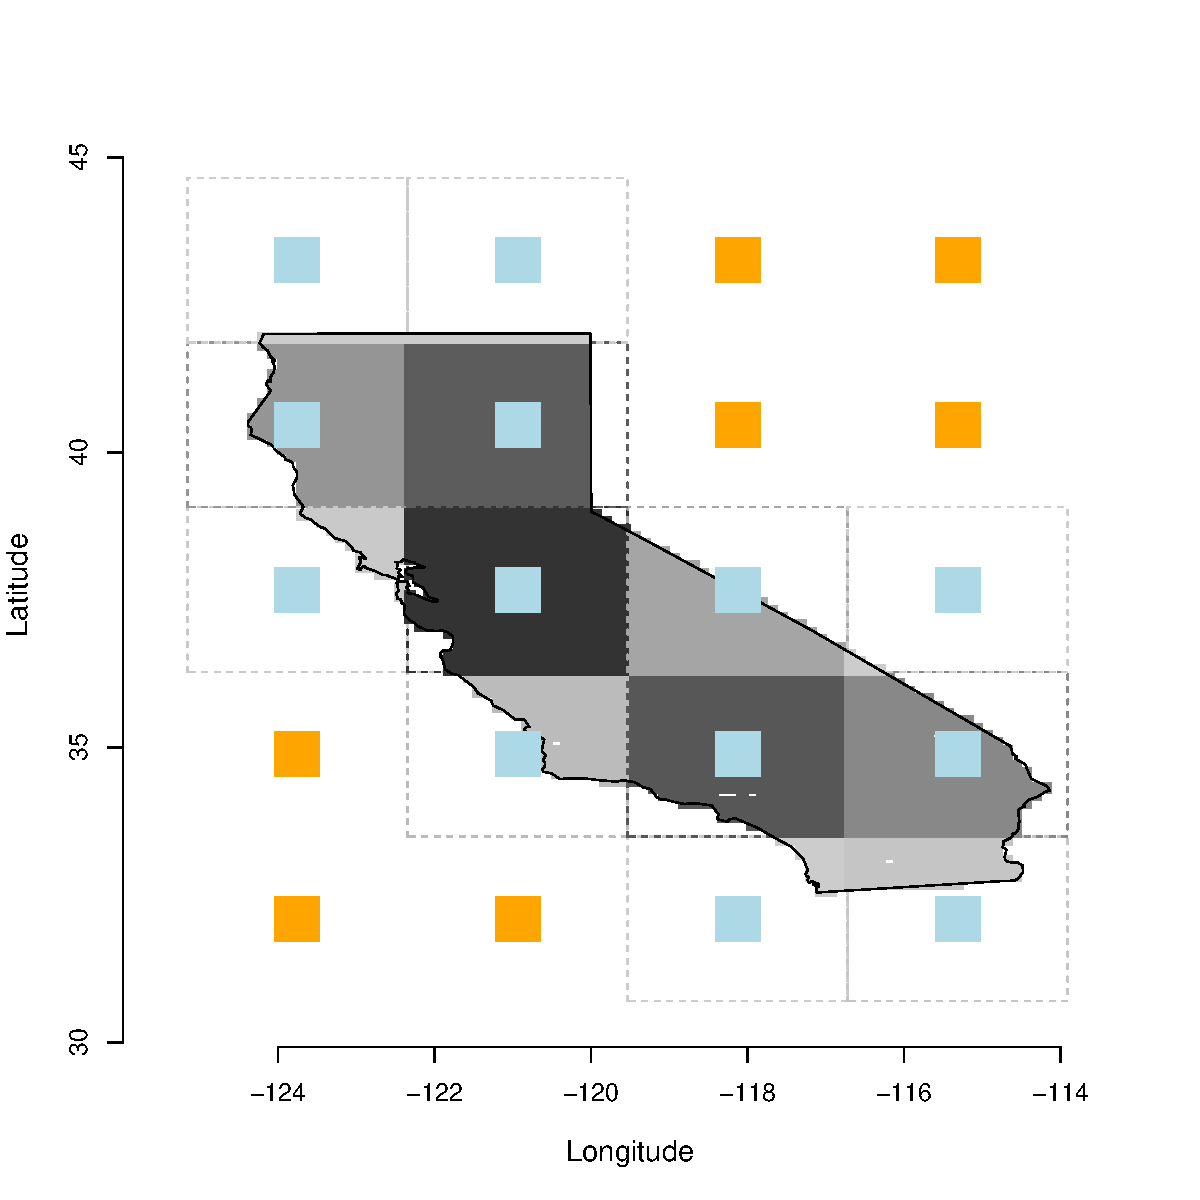
\includegraphics[scale=0.18]{figs/cal_mod_box3.pdf}
\end{center}
\caption{Left: CanCM4 simulation grid cells. Center: Observation locations. Right: method for computing weighted sum or average for CanCM4 to make values comparable with observations.}
\end{figure}

\end{frame}



\begin{frame}{DLM-based anomaly}
\begin{figure}
\begin{center}
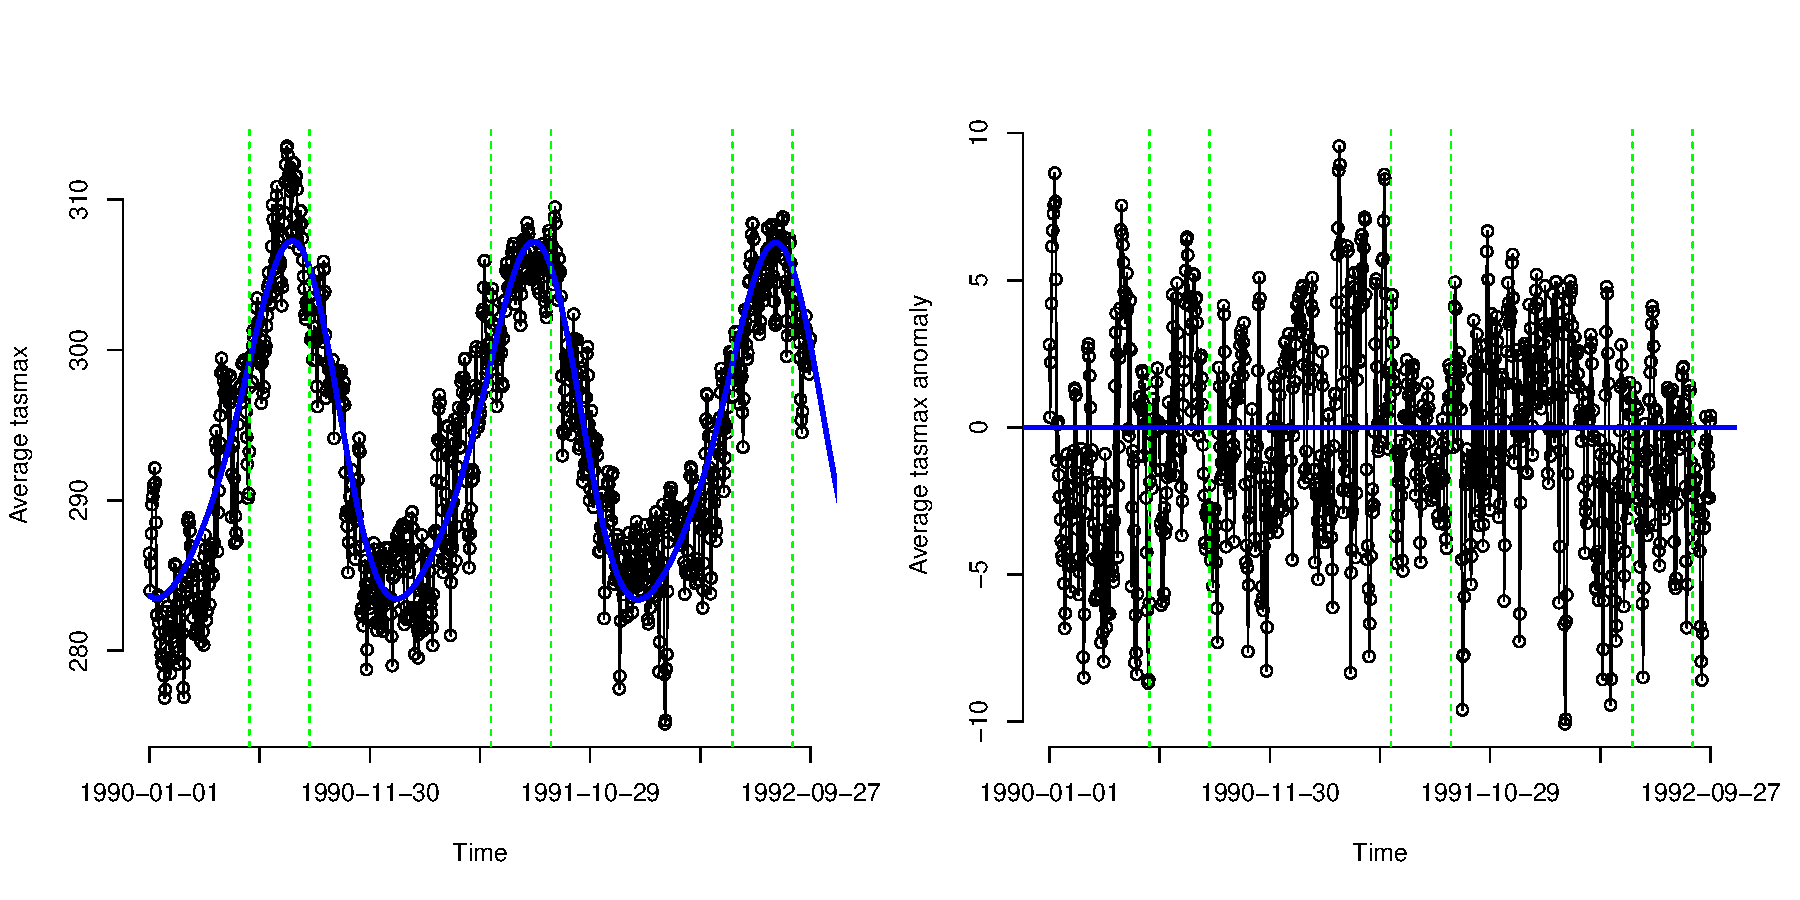
\includegraphics[scale=0.38]{figs/dlm.pdf}
\end{center}
\end{figure}
\end{frame}



\begin{frame}{Extremal index (declustering)}

The extremal index $\theta$ is the inverse of the limiting mean cluster size
\bigskip

It can be estimated using interexceedance times, $T_i = S_{i+1} - S_i$, with a log-likelihood of
\begin{align*}
l(\theta, p; \m{T}) =&~ m_1\log(1-\theta p^\theta) + (N-1-m_1)\{\log(\theta)+ \log(1-p^\theta)\} \nonumber \\
 &+ \theta\log(p)\sum_{i=1}^{N-1}(T_i-1)
\end{align*}
$p$ is the probability of not exceeding the threshold

\end{frame}



\begin{frame}{Declustering}
\begin{figure}
\begin{center}
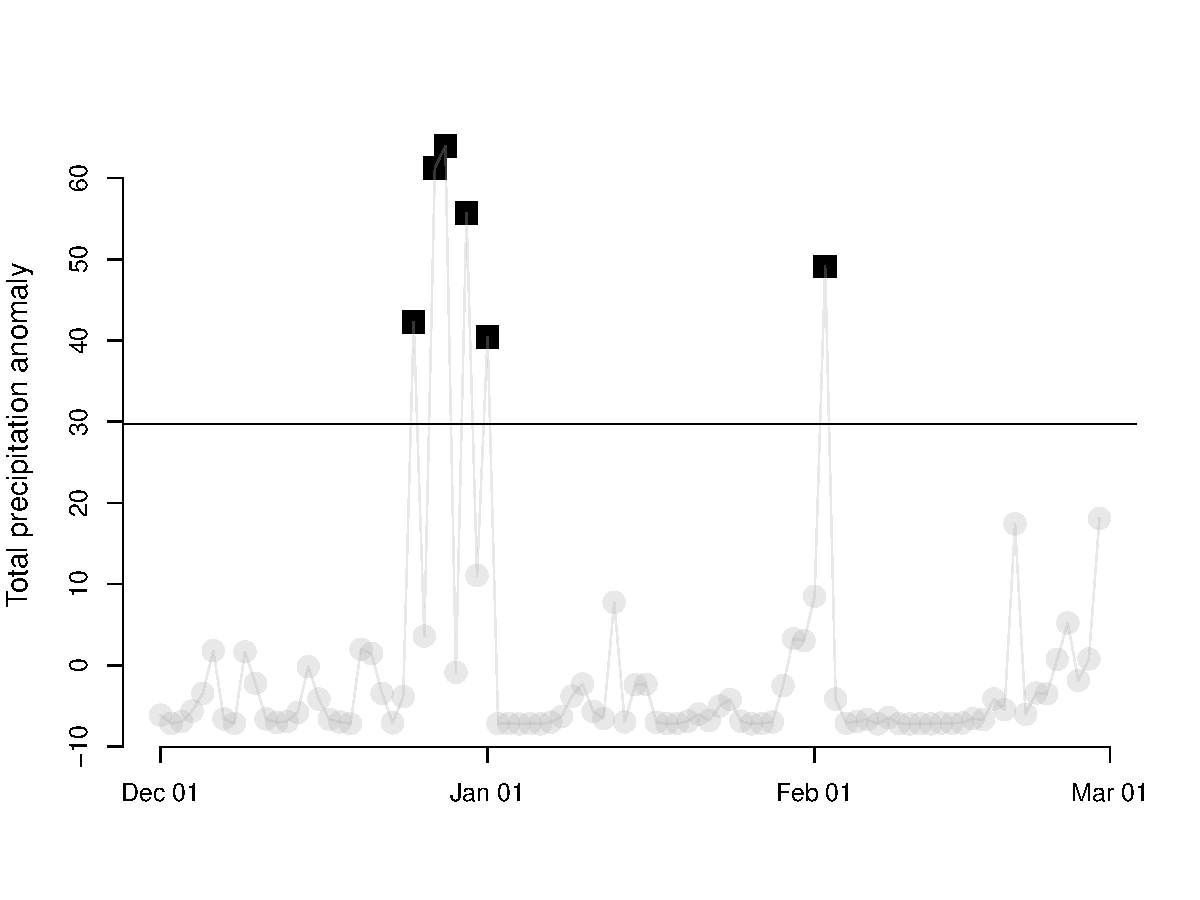
\includegraphics[scale=0.38]{figs/threshold.pdf}
\end{center}
\end{figure}
\end{frame}

% \begin{frame}{Hierarchical model for threshold exceedance}
% \noindent For the $j$th observation in replicate $i$, we assume
% \[ X_{ij} \overset{ind}\sim F_i,~~~~~i=1,\ldots,R,~~~~~j=1,\ldots,n_i. \]
% \noindent For fixed $u$ and each $i$, define the following sets:
% \[ A_i = \{j:x_{ij}\leq u\},~~~ A_i^c = \{j: x_{ij}>u\} \]
% where $|A_i|=n_i-k_i$ and $|A_i^c|=k_i$ with $k_i$ being the number of exceedances in replicate $i$.
% \bigskip
% 
% \noindent Finally, we define our exceedances as
% \[ y_{ij} = 0\cdot \ind_{(j \in A_i)} + (x_{ij}-u)\cdot \ind_{(j \in A_i^c)} \]
% \end{frame}
% 
% \begin{frame}{Likelihood}
% \noindent The likelihood is given by
% \begin{eqnarray*}
% L(\m{y}; \m{\sigma}, \m{\xi}, \m{\zeta}) &=& \prod_{i=1}^R f_{Y_i}(\m{y}_i|\sigma_i,\xi_i,\zeta_i) \\
% &=& \prod_{i=1}^R\left[\prod_{A_i} F_{X_i}(u) \times \prod_{A_i^c} f_{X_i}(y_{ij}+u)\right] \\
% &\approx& \prod_{i=1}^R\left[\prod_{A_i} F_{X_i}(u) \times \prod_{A_i^c} [1-F_{X_i}(u)]g(y_{ij}|\sigma_i,\xi_i)\right] \\
% &=& \prod_{i=1}^R\left[\prod_{A_i} (1-\zeta_i)\times \prod_{A_i^c} \frac{\zeta_i}{\sigma_i}\left(1+\xi_i\frac{y_{ij}}{\sigma_i}\right)_+^{-1/\xi_i-1}\right] \\
% \end{eqnarray*}
% 
% \end{frame}


\begin{frame}{Likelihood}

Replicate $i$, observation $j$, exceedances $Y_{ij} = X_{ij} - u$, and keep only those $Y_i > 0$. These have likelihood
\[ L(\m{y}; \m{\sigma}, \m{\xi}, \m{\zeta}) = \prod_{i=1}^R\left[(1-\zeta_i)^{n_i-k_i}\zeta_i^{k_i}\prod_{j=1}^{k_i}\frac{1}{\sigma_i}\left(1+\xi_i\frac{y_{ij}}{\sigma_i}\right)_+^{-1/\xi_i-1}\right] \]

$n_i$ is the number of $X_{ij}$'s

$k_i$ is the number of $Y_{ij}$'s

$\zeta_i$ is the probability of exceeding the threshold
% where $n_i$ is number of $X_{ij}$'s and $k_i$ is number of $Y_{ij}$'s, and $\zeta_i$ is the probability of exceeding the threshold

\end{frame}


\begin{frame}{Priors}
\noindent These priors complete the hierarchical model formulation. Greek letters are random variables while English letters are fixed.
\begin{eqnarray*}
\sigma_i|\alpha, \beta &\sim& Gamma(\alpha, \beta) \\
\xi_i|\xi, \tau^2  &\sim& Normal(\xi, \tau^2) \\
\zeta_i|\mu, \eta &\sim& Beta(\mu\eta, (1-\mu)\eta) \\
%\theta_i|\theta_\mu, \theta_\tau &\sim& Beta(\theta_\mu\theta_\tau, (1-\theta_\mu)\theta_\tau) \\
 \\
\alpha_\sigma \sim Gamma(a_\alpha, b_\alpha)&  &\beta_\sigma \sim Gamma(a_\beta, b_\beta) \\
\xi \sim Normal(m, s^2)&  &\tau^2 \sim Gamma(a_\tau, b_\tau) \\
\mu \sim Beta(a_\mu, b_\mu)&  &\eta \sim Gamma(a_\eta, b_\eta) \\
%\theta_\mu \sim Beta(a_{\theta_\mu}, b_{\theta_\mu})&  &\theta_\tau \sim Gamma(a_{\theta_\tau}, b_{\theta_\tau})
\end{eqnarray*}

\end{frame}



\begin{frame}{Return level}

For a distribution $G$, the return level $x_m$ is the solution to
\[ G(x_m) = 1-\frac{1}{m}. \]
The value $x_m$ is exceeded on average once every $m$ observations.
\bigskip

For the GPD, the return level is given by
\[ x_m = u +\frac{\sigma}{\xi}\left[\left(m\zeta\theta\right)^\xi-1\right] \]



\end{frame}




\begin{frame}{Bhattacharyya distance}

Bhattacharyya coefficient
\[ BC(p,q)=\int_\mathcal{X} \sqrt{p(x)q(x)} dx \]

Bhattacharyya distance
\[ D_B(p,q)=-\log BC(p,q). \]

$D_B$ is computed between parameters in the replicates (and observations) and parameters in the hierarchy.

\end{frame}



\begin{frame}
\begin{center}
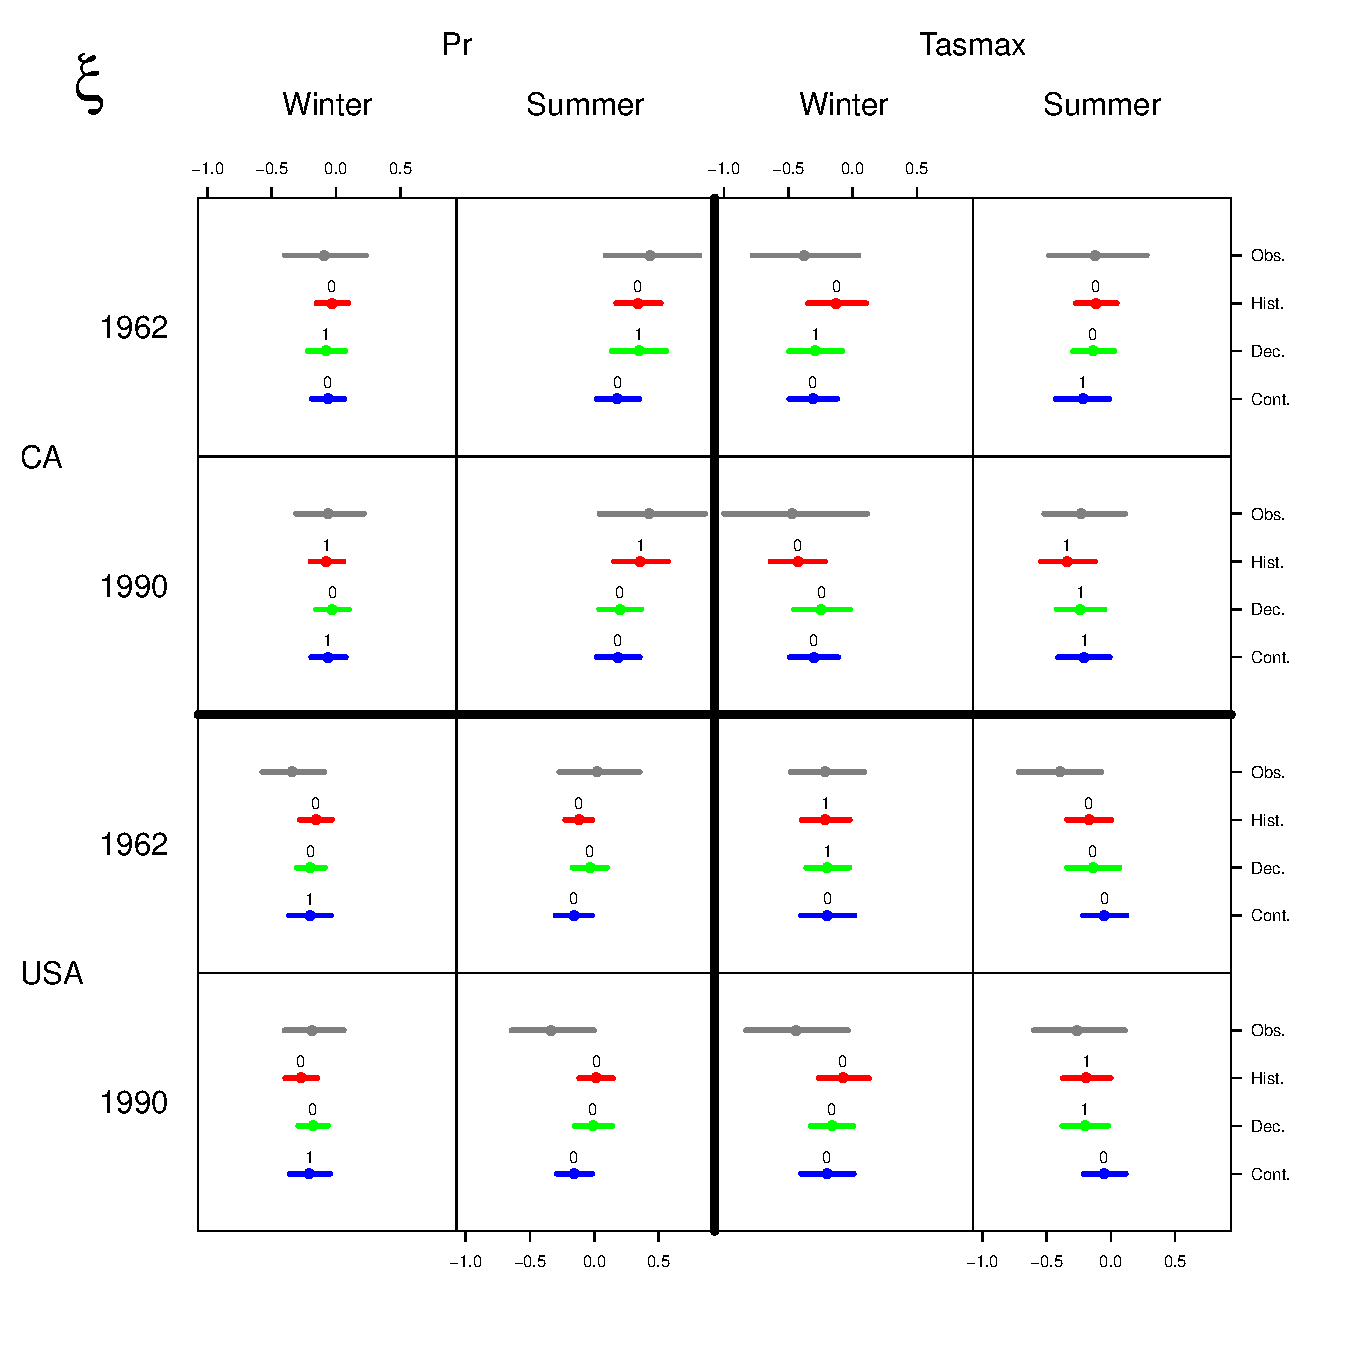
\includegraphics[scale=0.34]{figs/shape.pdf}
\end{center}
\end{frame}

\begin{frame}
\begin{center}
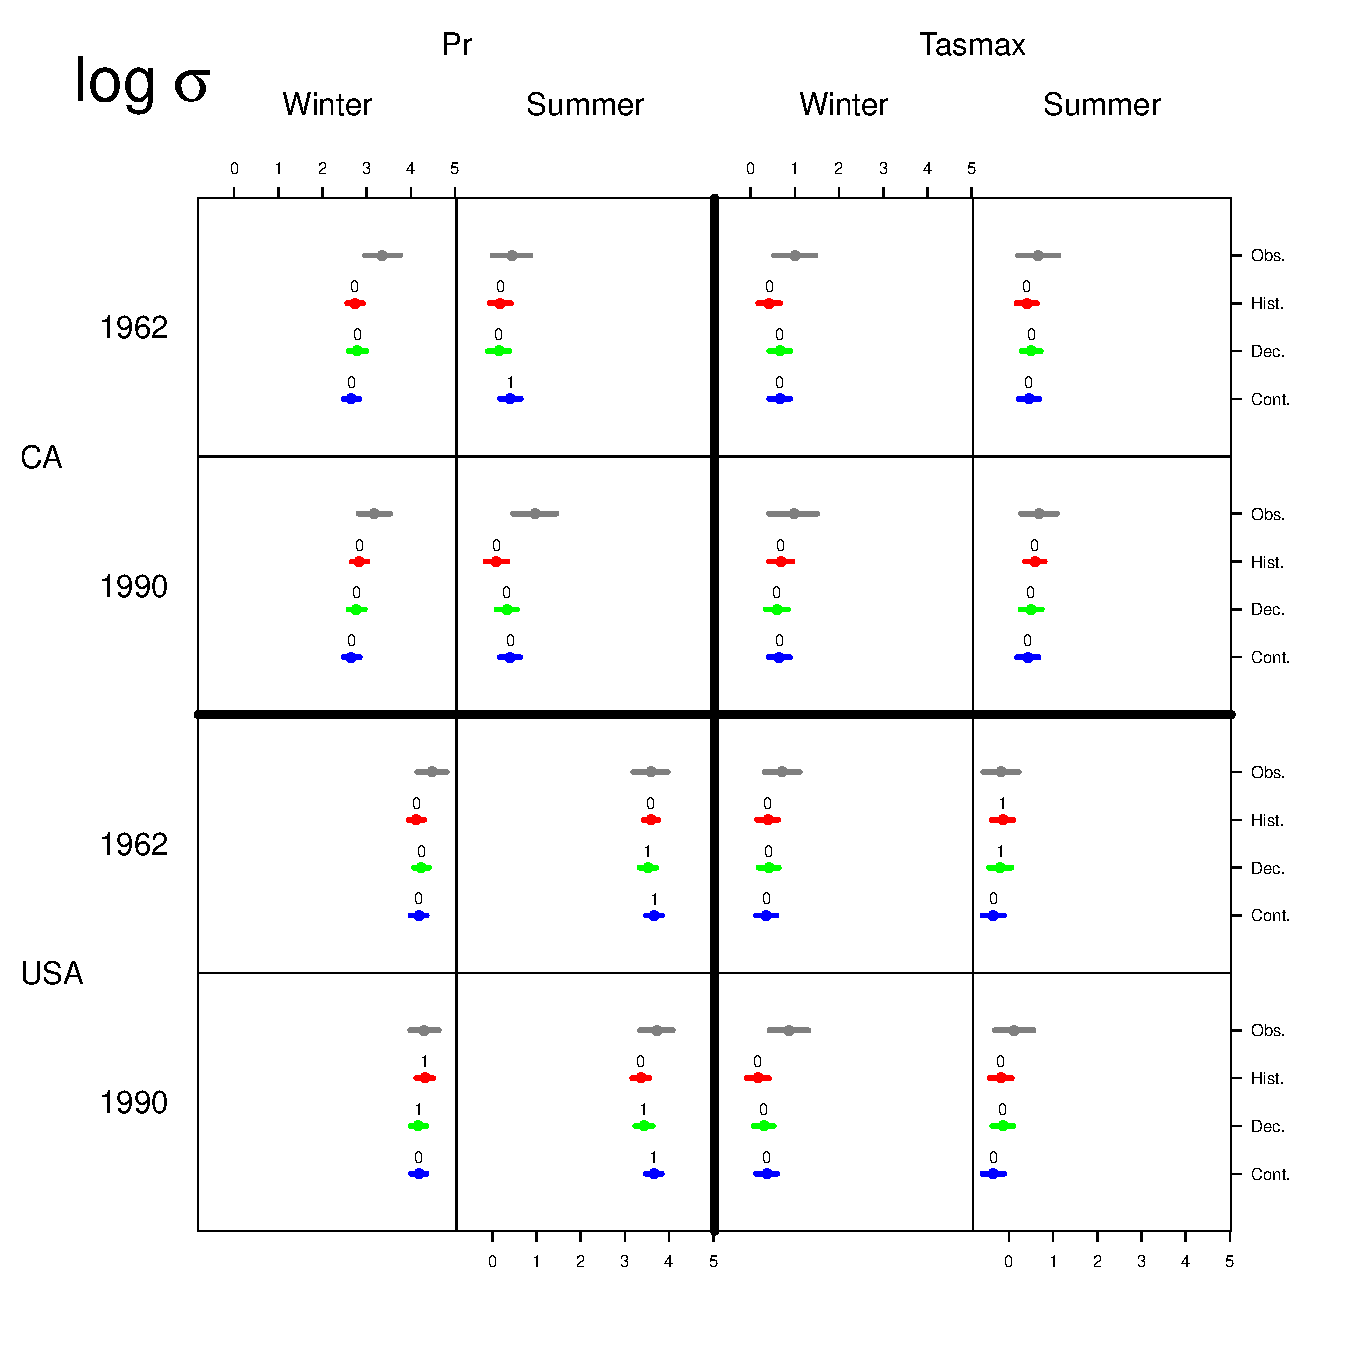
\includegraphics[scale=0.34]{figs/log_sigma.pdf}
\end{center}
\end{frame}

\begin{frame}
\begin{center}
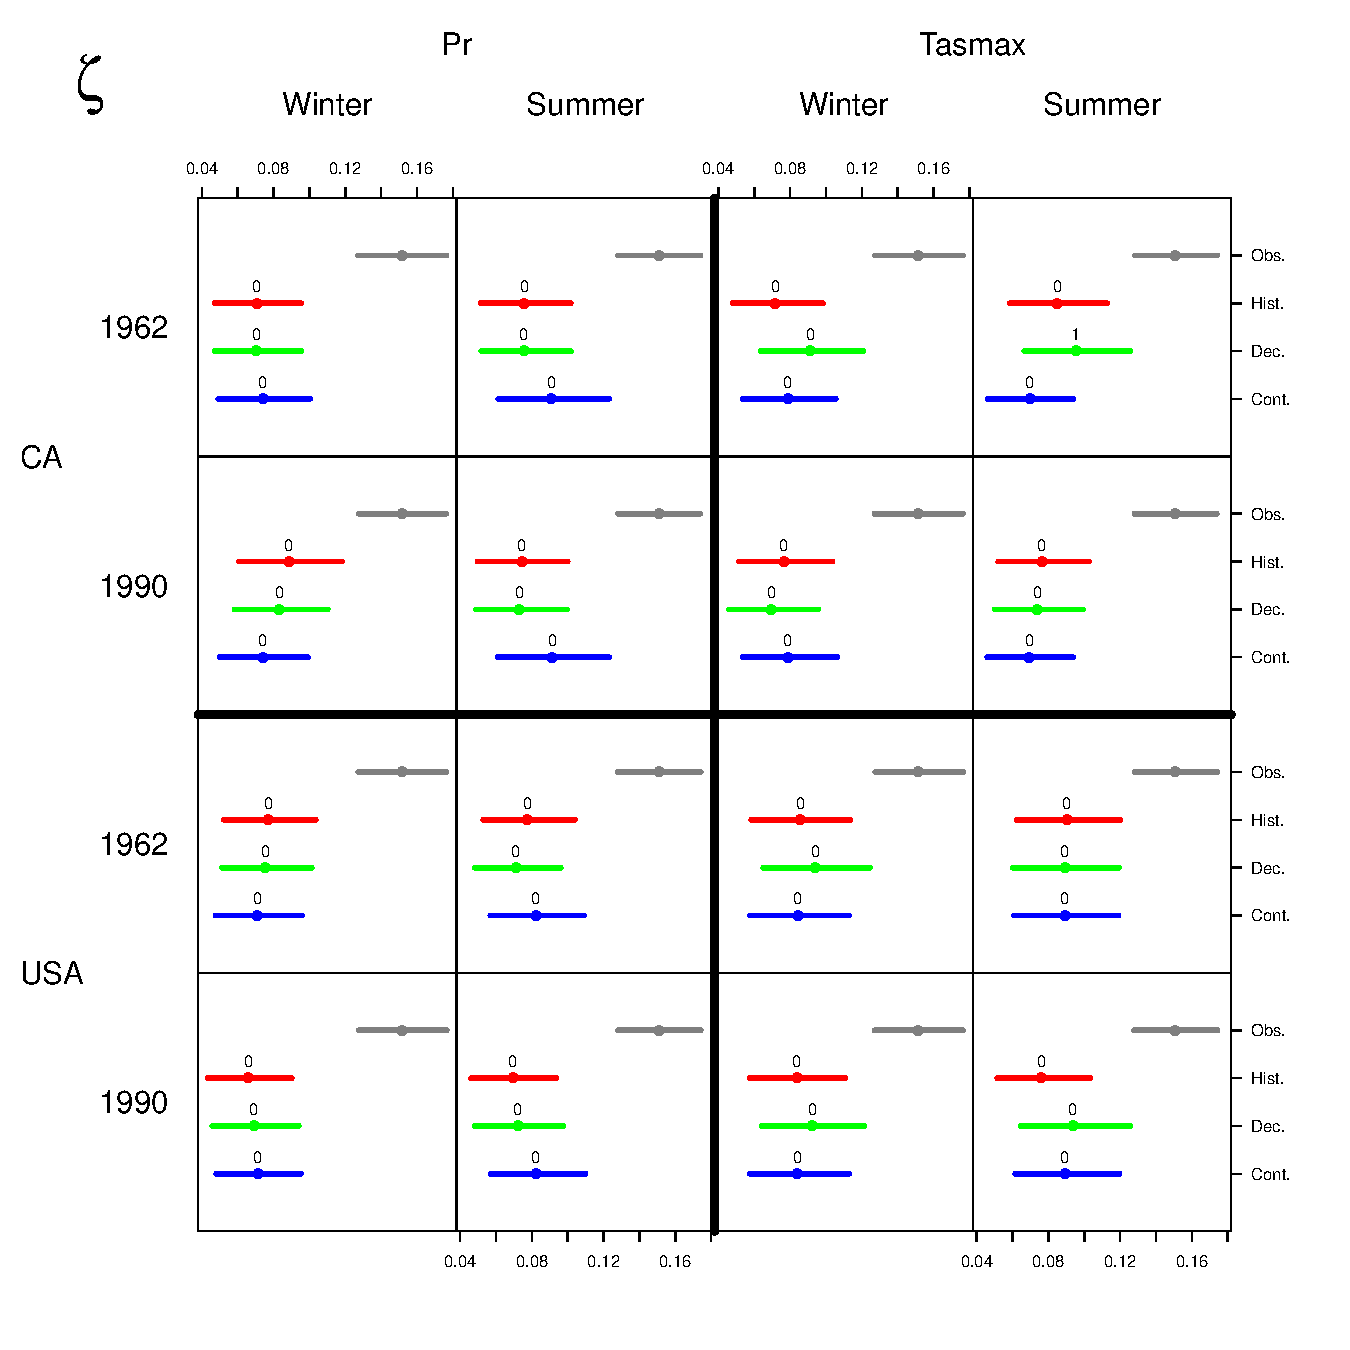
\includegraphics[scale=0.34]{figs/zeta.pdf}
\end{center}
\end{frame}

\begin{frame}
\begin{center}
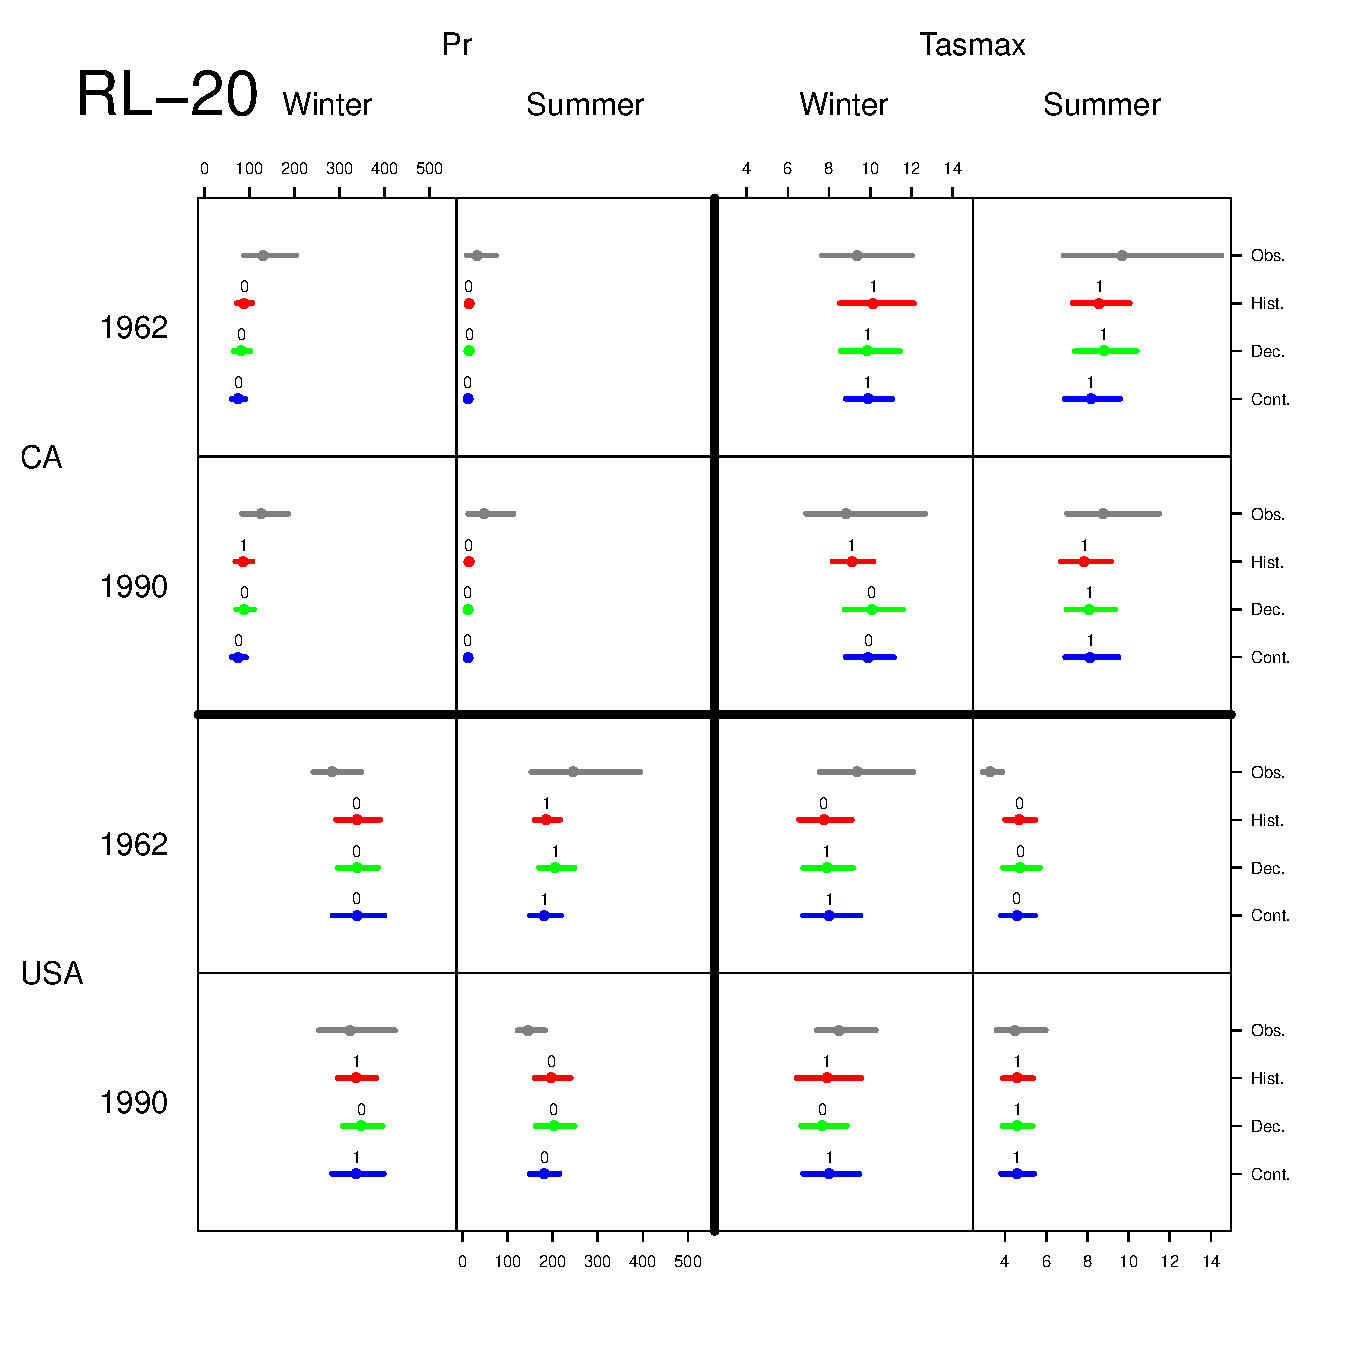
\includegraphics[scale=0.34]{figs/rl20.pdf}
\end{center}
\end{frame}

\begin{frame}
\begin{center}
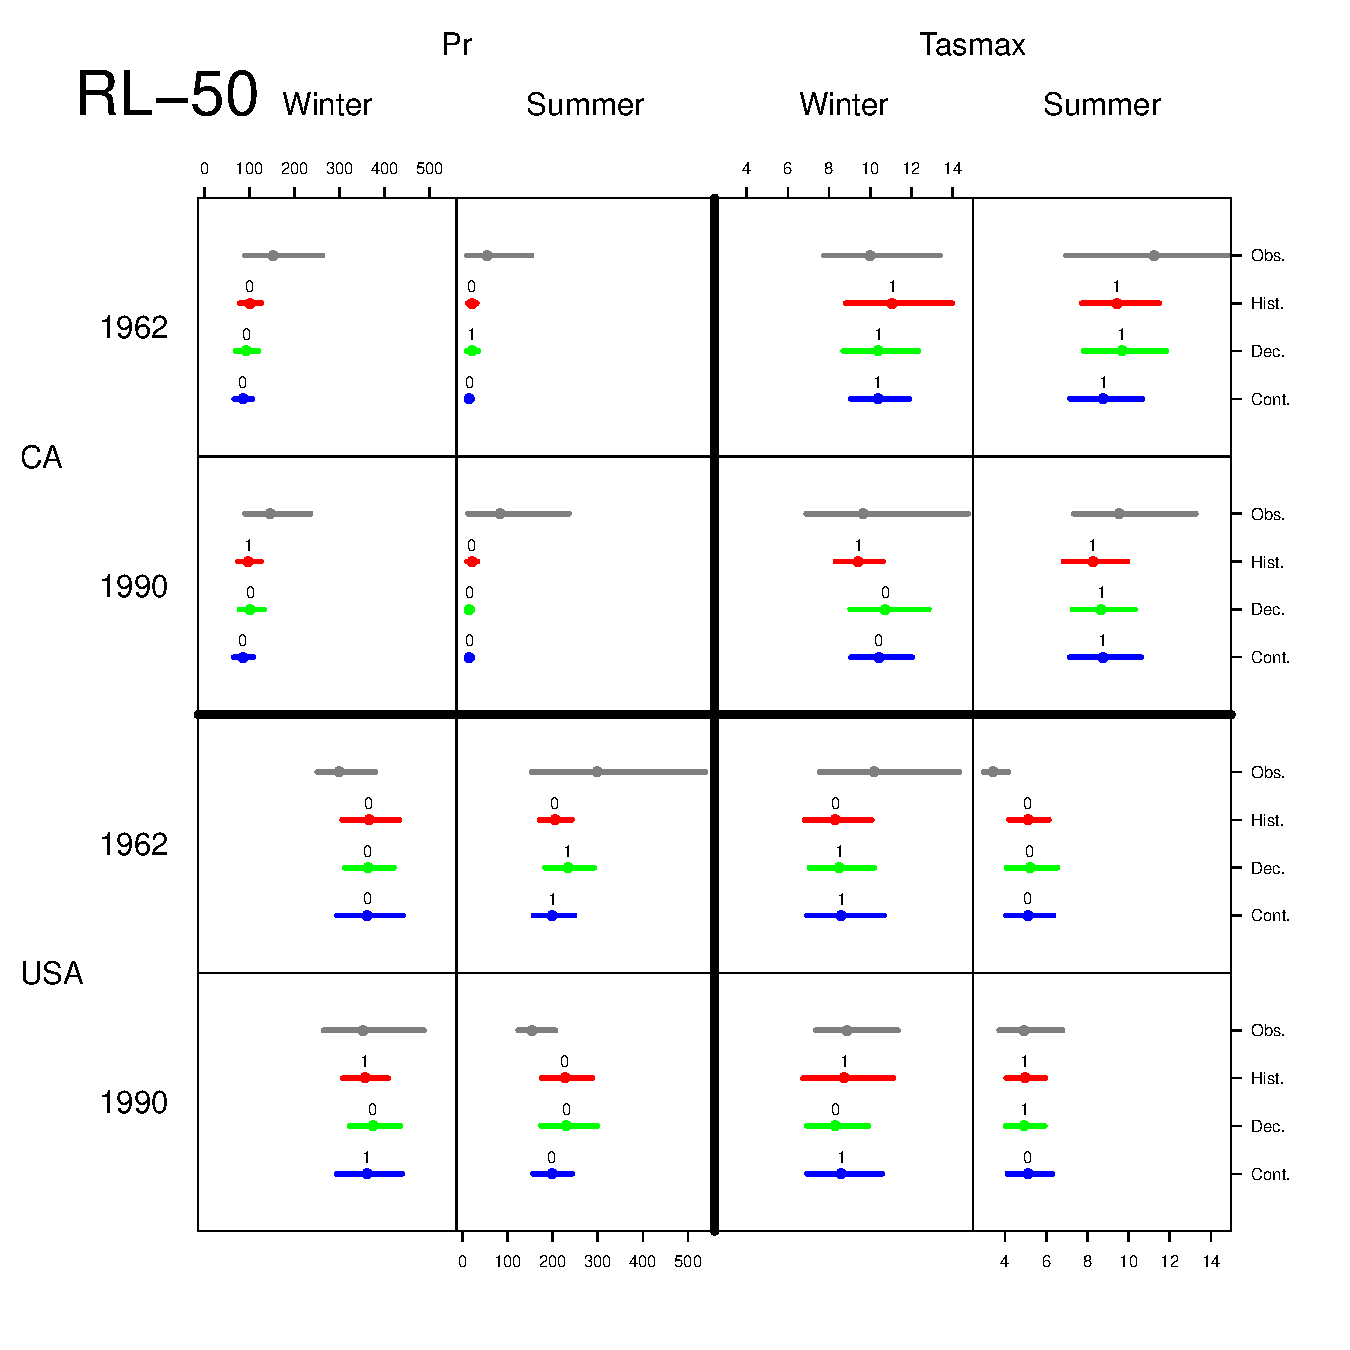
\includegraphics[scale=0.34]{figs/rl50.pdf}
\end{center}
\end{frame}

\begin{frame}
\begin{center}
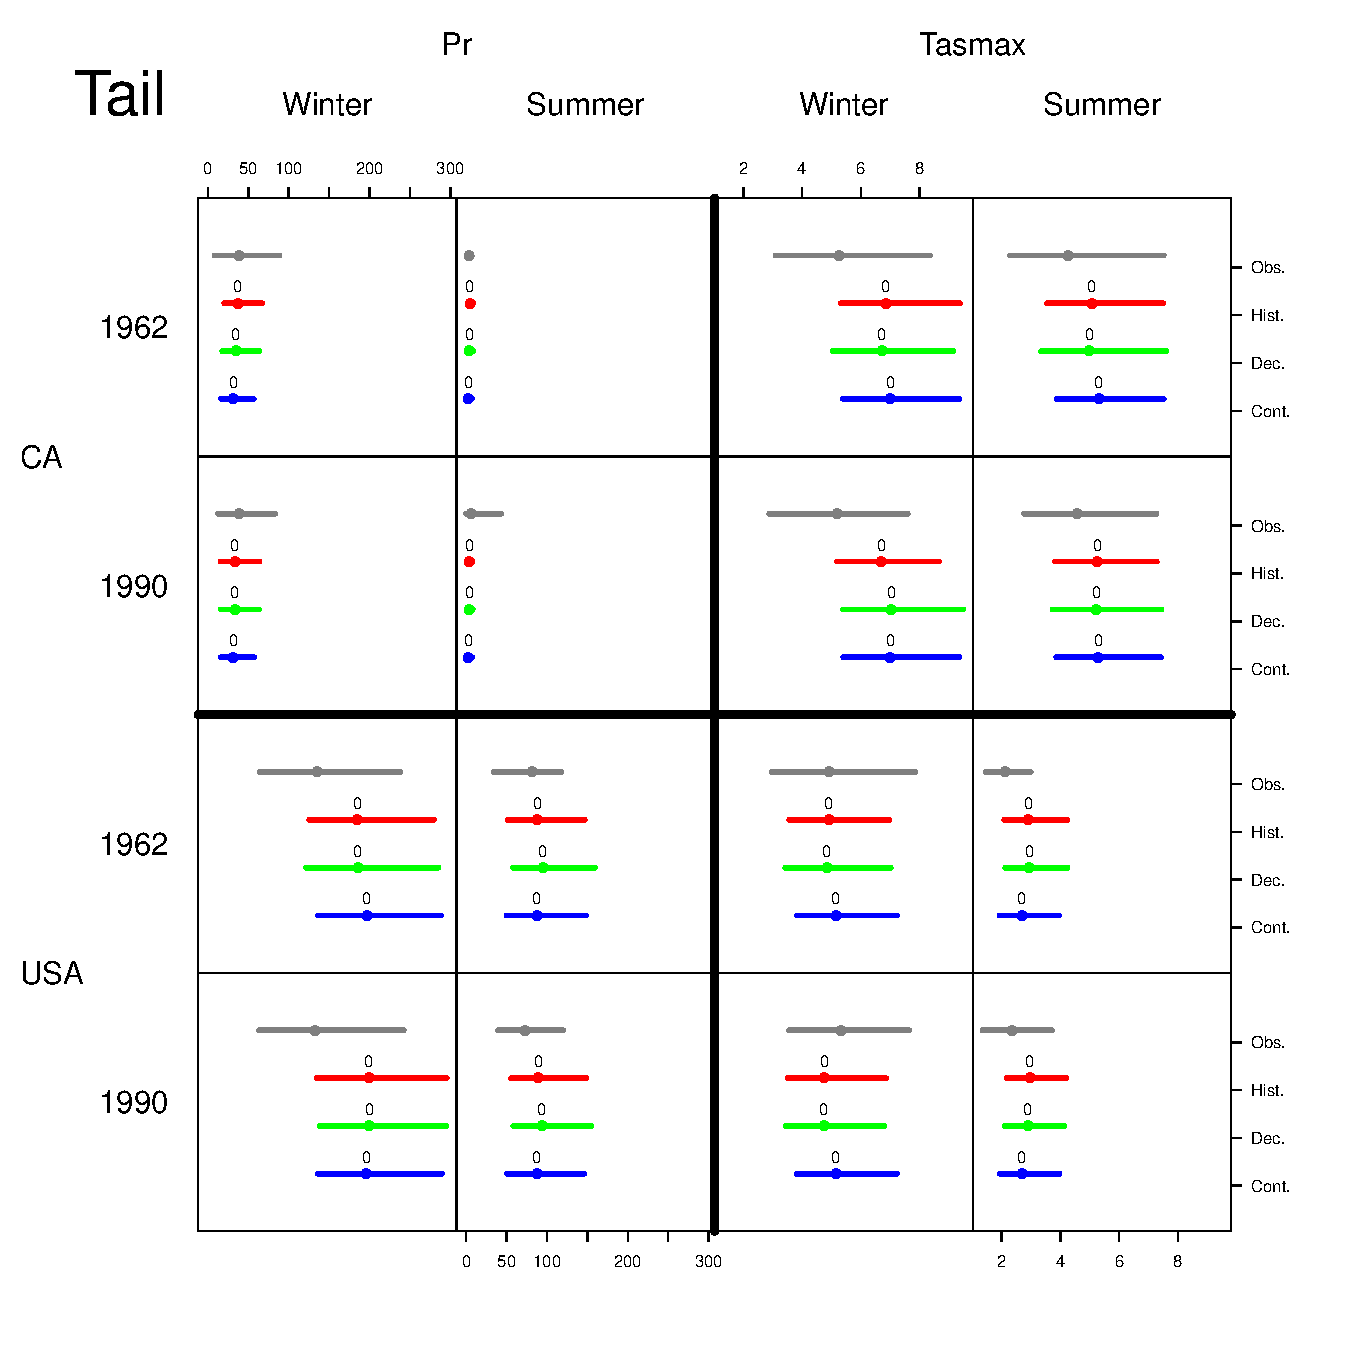
\includegraphics[scale=0.34]{figs/gp_tail.pdf}
\end{center}
\end{frame}

\begin{frame}
\begin{center}
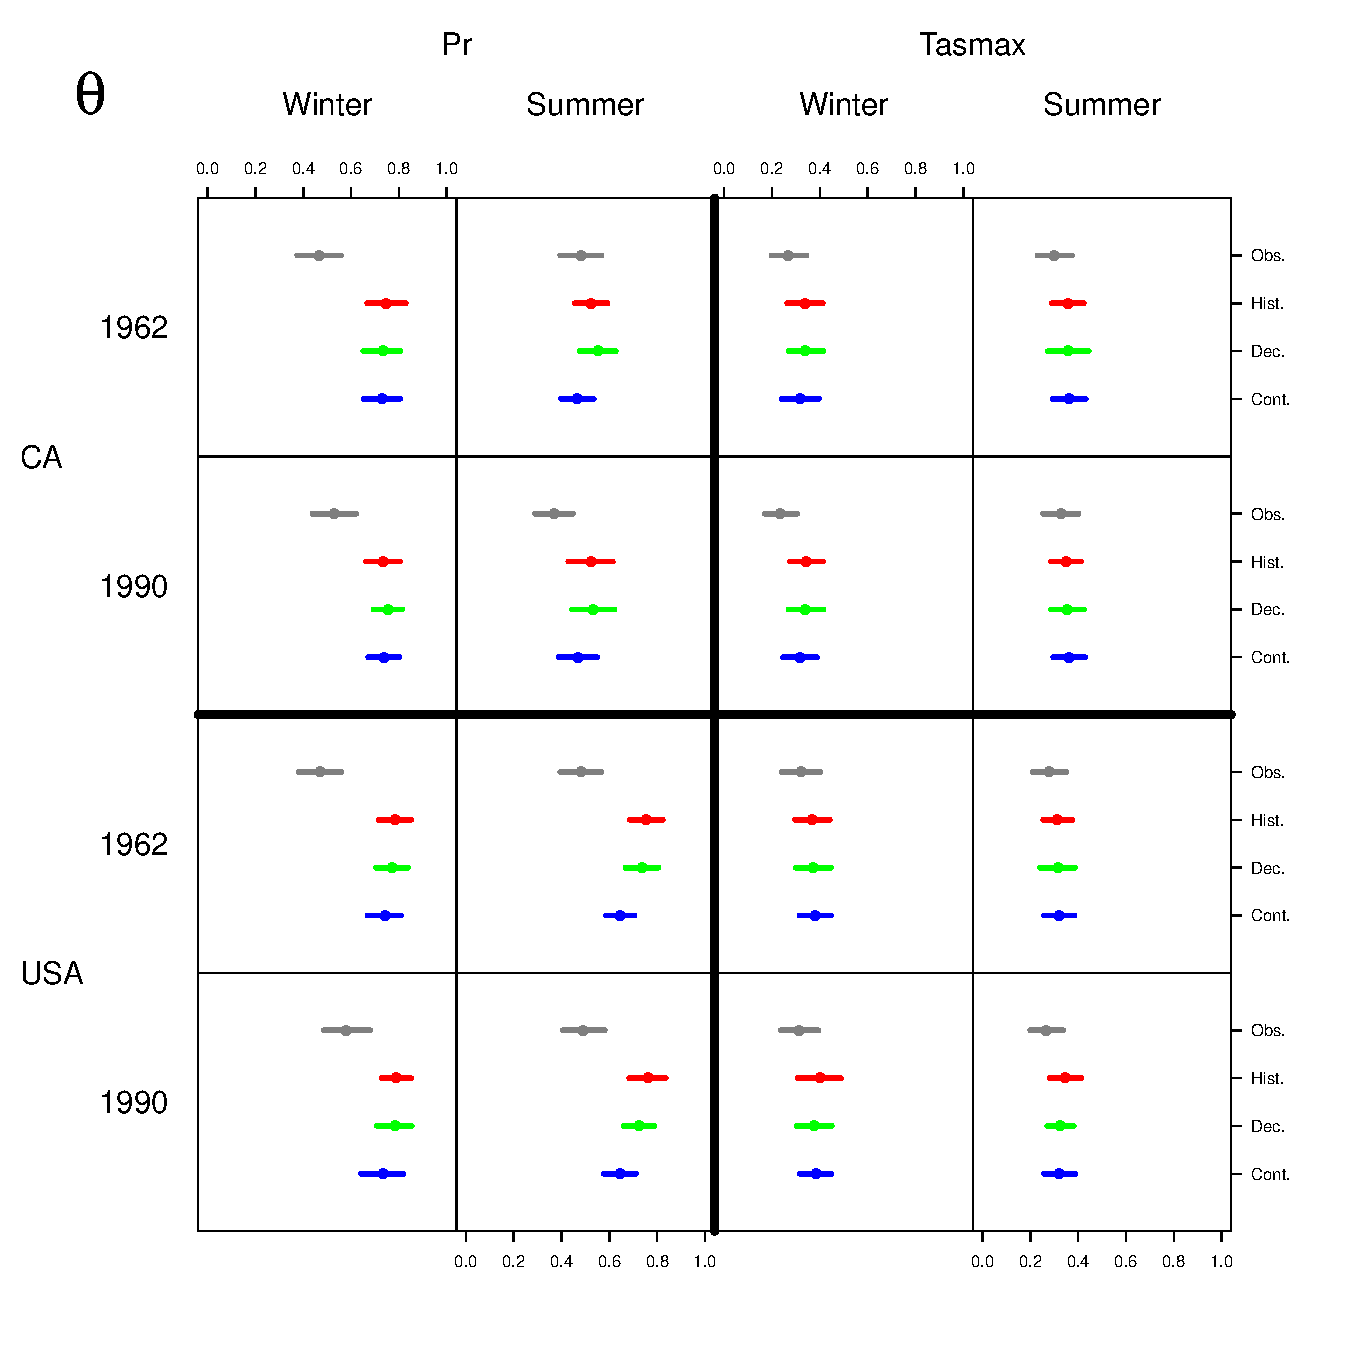
\includegraphics[scale=0.34]{figs/theta.pdf}
\end{center}
\end{frame}


\begin{frame}{Bivariate analysis}

Bivariate analysis using simple Pareto processes

\end{frame}

\begin{frame}{Simple pareto process}

Limit

Transform

Figure of transformed (include supremum cone) and non-transformed data

\end{frame}

\begin{frame}{}
\end{frame}

\begin{frame}
\begin{center}
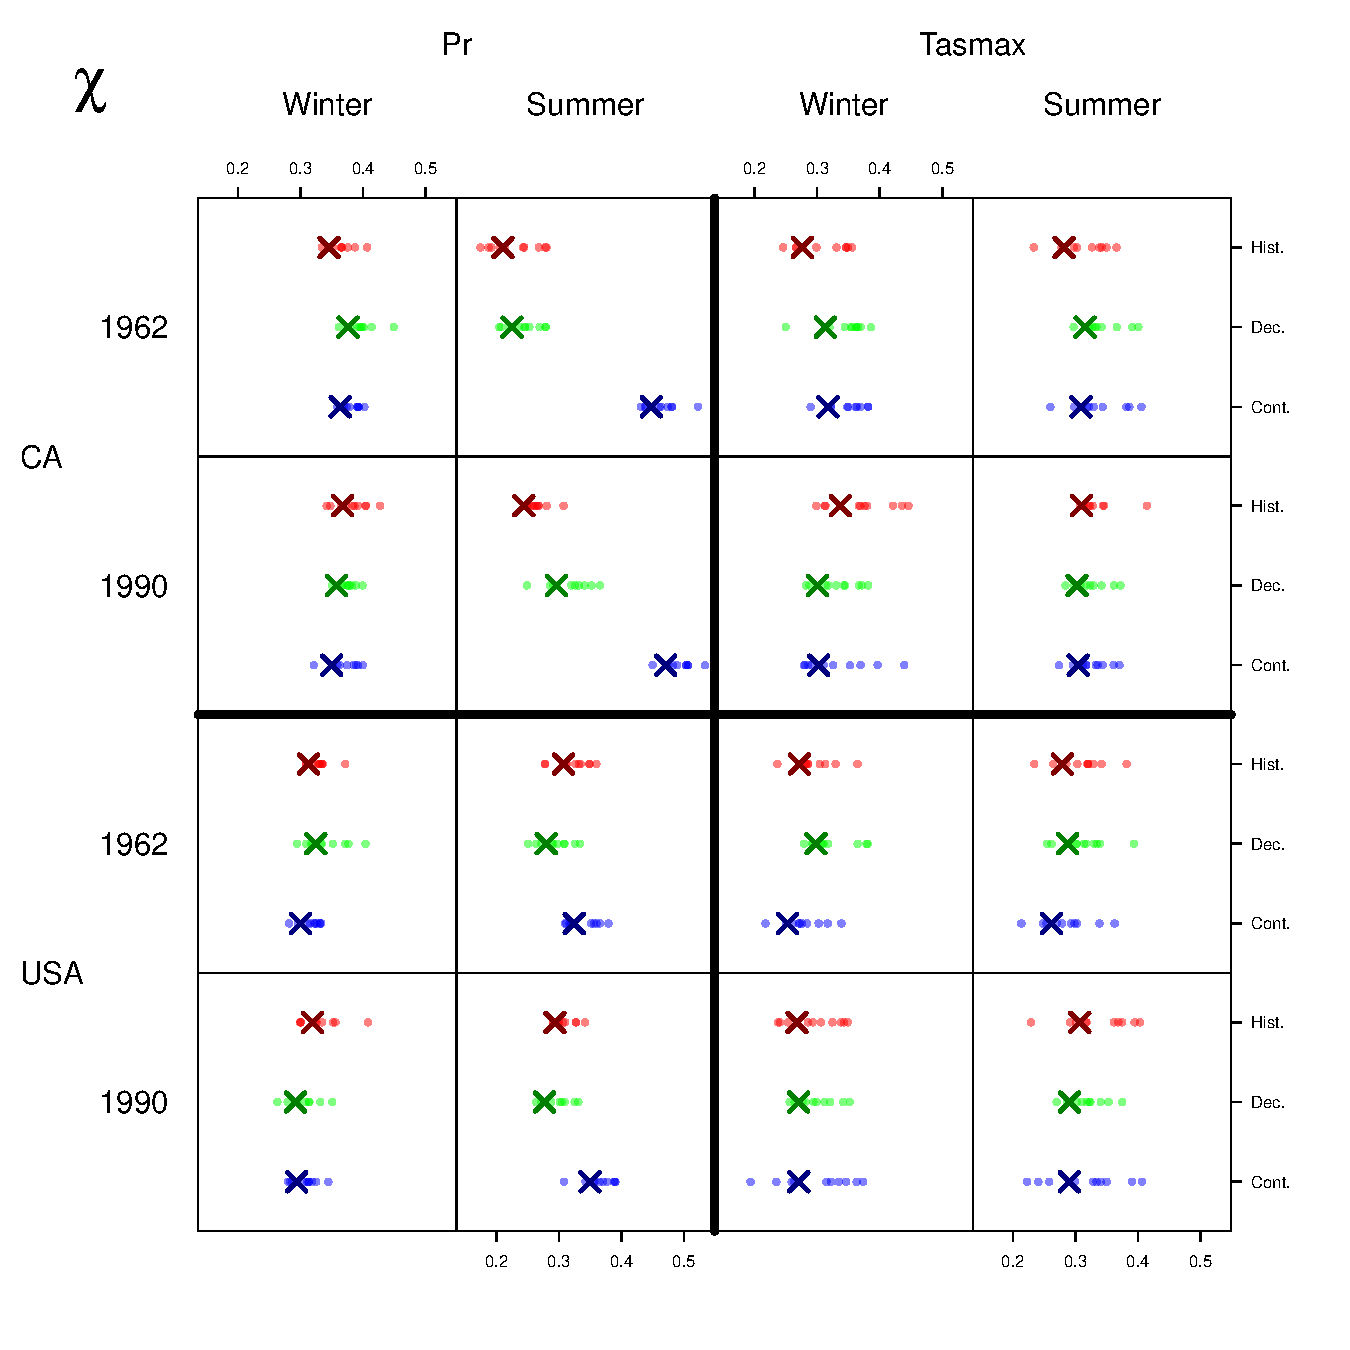
\includegraphics[scale=0.34]{figs/chi4.pdf}
\end{center}
\end{frame}





% 
% 
% \begin{frame}
% \begin{center}
% \includegraphics[scale=0.28]{figs/decadal1961_california_winter_pr_hier_zeta.pdf}
% \end{center}
% \end{frame}
% 
% \begin{frame}
% \begin{center}
% \includegraphics[scale=0.28]{figs/decadal1961_california_winter_pr_hier_returnlevel.pdf}
% \end{center}
% \end{frame}
% 
% \begin{frame}
% \begin{center}
% \includegraphics[scale=0.28]{figs/decadal1989_california_winter_pr_hier_ksi.pdf}
% \end{center}
% \end{frame}
% 
% 
% \begin{frame}
% \begin{center}
% \includegraphics[scale=0.28]{figs/decadal1989_california_winter_pr_hier_sigma.pdf}
% \end{center}
% \end{frame}
% 
% 
% \begin{frame}
% \begin{center}
% \includegraphics[scale=0.28]{figs/decadal1989_california_winter_pr_hier_zeta.pdf}
% \end{center}
% \end{frame}
% 
% \begin{frame}
% \begin{center}
% \includegraphics[scale=0.28]{figs/decadal1989_california_winter_pr_hier_returnlevel.pdf}
% \end{center}
% \end{frame}
% 
% 
% \begin{frame}
% \begin{center}
% \includegraphics[scale=0.28]{figs/decadal1961_usa_winter_pr_hier_ksi.pdf}
% \end{center}
% \end{frame}
% 
% 
% \begin{frame}
% \begin{center}
% \includegraphics[scale=0.28]{figs/decadal1961_usa_winter_pr_hier_sigma.pdf}
% \end{center}
% \end{frame}
% 
% 
% \begin{frame}
% \begin{center}
% \includegraphics[scale=0.28]{figs/decadal1961_usa_winter_pr_hier_zeta.pdf}
% \end{center}
% \end{frame}
% 
% \begin{frame}
% \begin{center}
% \includegraphics[scale=0.28]{figs/decadal1961_usa_winter_pr_hier_returnlevel.pdf}
% \end{center}
% \end{frame}
% 
% \begin{frame}
% \begin{center}
% \includegraphics[scale=0.28]{figs/decadal1989_usa_winter_pr_hier_ksi.pdf}
% \end{center}
% \end{frame}
% 
% 
% \begin{frame}
% \begin{center}
% \includegraphics[scale=0.28]{figs/decadal1989_usa_winter_pr_hier_sigma.pdf}
% \end{center}
% \end{frame}
% 
% 
% \begin{frame}
% \begin{center}
% \includegraphics[scale=0.28]{figs/decadal1989_usa_winter_pr_hier_zeta.pdf}
% \end{center}
% \end{frame}
% 
% \begin{frame}
% \begin{center}
% \includegraphics[scale=0.28]{figs/decadal1989_usa_winter_pr_hier_returnlevel.pdf}
% \end{center}
% \end{frame}

\end{document}
